%\documentclass[notes]{beamer}       			% compila sia i frame che le note
\documentclass{beamer}              			% compila solo i frame
%\documentclass[notes=only]{beamer}  	% compila solo le note

% ita language and encoding
\usepackage[utf8]{inputenc}
\usepackage[italian]{babel}

% formattazione
\usepackage{ragged2e} 							% pacchetto che contiene il comando \justifying
\apptocmd{\frame}{}{\justifying}{}  	% --> applica la giustificazione a tutti i frame del documento
%\justifying											% --> applica la giustificazione a tutto il documento

% graphics style
\usepackage{graphicx}
\usepackage{xcolor}
\usepackage{shadowtext}

%image paths
\graphicspath{{./Immagini/}{./Immagini/TRD/}}

% impostazioni base delle slide - tema, colori, caratteri, ... (deic.uab.es/~iblanes/beamer_gallery/)
\mode<presentation>
{
	\usetheme{CambridgeUS}      % or try Darmstadt, Madrid, Warsaw, ...
  	\usecolortheme{rose} 			% or try albatross, beaver, crane, orchid, rose ...
	\usefonttheme{structurebold} % or try structureitalicserif, structuresmallcapsserif
}

% settagio dati principali del file - titolo, autore, ...
\title[Presentation on the AMS-02 experiment]{The AMS-02 experiment}
\subtitle{General review of the apparatus}
\author{Daniele Di Bari}
\institute{University of Perugia}
\date{27th April 2017}
\subject{Course of Particle Detectors}

% By default the beamer class adds navigation buttons in the bottom right corner. To remove them one can place
\beamertemplatenavigationsymbolsempty

% settaggio prima slide
\setbeamertemplate{title page}
{
	\shadowcolor{white!30!black}
	\vspace{-0.5cm}	
	
    \shadowtext{\textcolor{white}{\textbf{\footnotesize{The Alpha Magnetic Spectrometer}}}}
   
    \vspace{0.15cm}  	
    
   	\shadowtext{\textcolor{white}{\textbf{\LARGE \inserttitle}}}\par
      
   	\vspace{0.1cm}  

   	\shadowtext{\textcolor{white}{\emph{\large \insertsubtitle}}}\par
   	
   	\vspace{2.5cm}
	
	\titlepagetext{lightgray}{The general particle physics}\\
	\titlepagetext{lightgray}{experiment in space, on board}\\
	\titlepagetext{lightgray}{the International Space Station}\\
	\titlepagetext{lightgray}{since 19th May 2011.}		
}
				
% colors
\definecolor{itemred}{RGB}{163,0,0}
\definecolor{itemblue}{RGB}{52,57,176}

% COMANDI
% Formato testo generico in titolpage
\newcommand\titlepagetext[2]{\textcolor{#1}{\footnotesize{\textit{{#2}}}}}
\newcommand\colortextbf[2]{\textcolor{#1}{\textbf{#2}}}
\newcommand\bluetextbf[1]{\textcolor{itemblue}{\textbf{#1}}}
\newcommand\bluetextit[1]{\textcolor{itemblue}{\textit{#1}}}
\newcommand\textitem[2]{\textcolor{itemblue}{\textbf{#1} (\textit{#2})}}

% Testo giustificato
\newenvironment<>{justify}{\justifying{}}


% 	MODIFICA DEL TEMA CambridgeUS -- HEAD AND FOOTLINES
%		Il tema CambridgeUS usa il outer-tema "infolines" outer theme che imposta head and footlines (vedi il file .sty: ../tex/latex/beamer/themes/theme/beamerthemeCambridgeUS.sty). 
%		Ad esempio, in "beamerouterthemeinfolines.sty" è definito il "footline template" in cui sono dichiarate tre caselle - la prima per l'autore, la seconda per il titolo e l'ultima per la data e il numero.
%		Utilizzo delle impostazioni di base di "infolines" e modificando diversi parametri per ottenere il layout il tema personalizzato
\setbeamercolor{institute in head/foot}{parent=palette secondary}
\setbeamercolor{subject in head/foot}{parent=palette tertiary}
\setbeamercolor{title in head/foot}{parent=palette primary}
\setbeamertemplate{footline}
{
	\leavevmode%
	\hbox{%
  		% "ht" è lo spazio sopra il carattere partendo dalla base del carattere, "dp"  è lo spazio sotto il carattere partendo sempre dalla base del carattere
  		\begin{beamercolorbox}[wd=.333333\paperwidth,ht=2.5ex,dp=1ex,left,leftskip=4ex]{author in head/foot}%
   			\usebeamerfont{author in head/foot}\insertshortauthor
  		\end{beamercolorbox}%
  		\begin{beamercolorbox}[wd=.333333\paperwidth,ht=2.5ex,dp=1ex,center]{institute in head/foot}%
    		\usebeamerfont{title in head/foot}\insertshortinstitute
 		 \end{beamercolorbox}%
 		 \begin{beamercolorbox}[wd=.333333\paperwidth,ht=2.5ex,dp=1ex,right,rightskip=4ex]{date in head/foot}%
 		 	\usebeamerfont{date in head/foot}\insertshortdate{}\hspace*{2em}\insertframenumber{} / \inserttotalframenumber
 		 \end{beamercolorbox}
 		 }%
 	\vskip0pt%
}
\makeatletter
\setbeamertemplate{headline}
{
  \leavevmode%
  \hbox{%
  \begin{beamercolorbox}[wd=.5\paperwidth,ht=2.8ex,dp=1.35ex,left]{subject in head/foot}	
    \usebeamerfont{section in head/foot}\hspace*{4ex}Course of Particle Detectors			% --> N.B. Qui c'è l'unica scritta che non usa nessun template tipo \title o \institute
  \end{beamercolorbox}%
  \begin{beamercolorbox}[wd=.5\paperwidth,ht=2.8ex,dp=1.35ex,right]{title in head/foot}%
    \usebeamerfont{subsection in head/foot}\insertshorttitle\hspace*{4ex}
  \end{beamercolorbox}}%
  \vskip0pt%
}
\makeatother
%\makeatletter
%\setbeamertemplate{headline}
%{
%  \leavevmode%
%  \hbox{%
%  \begin{beamercolorbox}[wd=.5\paperwidth,ht=2.65ex,dp=1.5ex,right]{subject in head/foot}%
%    \usebeamerfont{section in head/foot}\expandafter\beamer@ifempty\expandafter{\insertsectionhead}{Course of Particle Detectors}{\insertsectionhead}\hspace*{2ex}
%  \end{beamercolorbox}%
%  \begin{beamercolorbox}[wd=.5\paperwidth,ht=2.65ex,dp=1.5ex,left]{title in head/foot}%
%    \usebeamerfont{subsection in head/foot}\hspace*{2ex}\expandafter\beamer@ifempty\expandafter{\insertsubsectionhead}{\insertshorttitle}{\insertsubsectionhead}
%  \end{beamercolorbox}}%
%  \vskip0pt%
%}
%\makeatother
%% FINE MODIFICA

\begin{document}
	% impostare una foto come sfondo del frame: 
	\usebackgroundtemplate{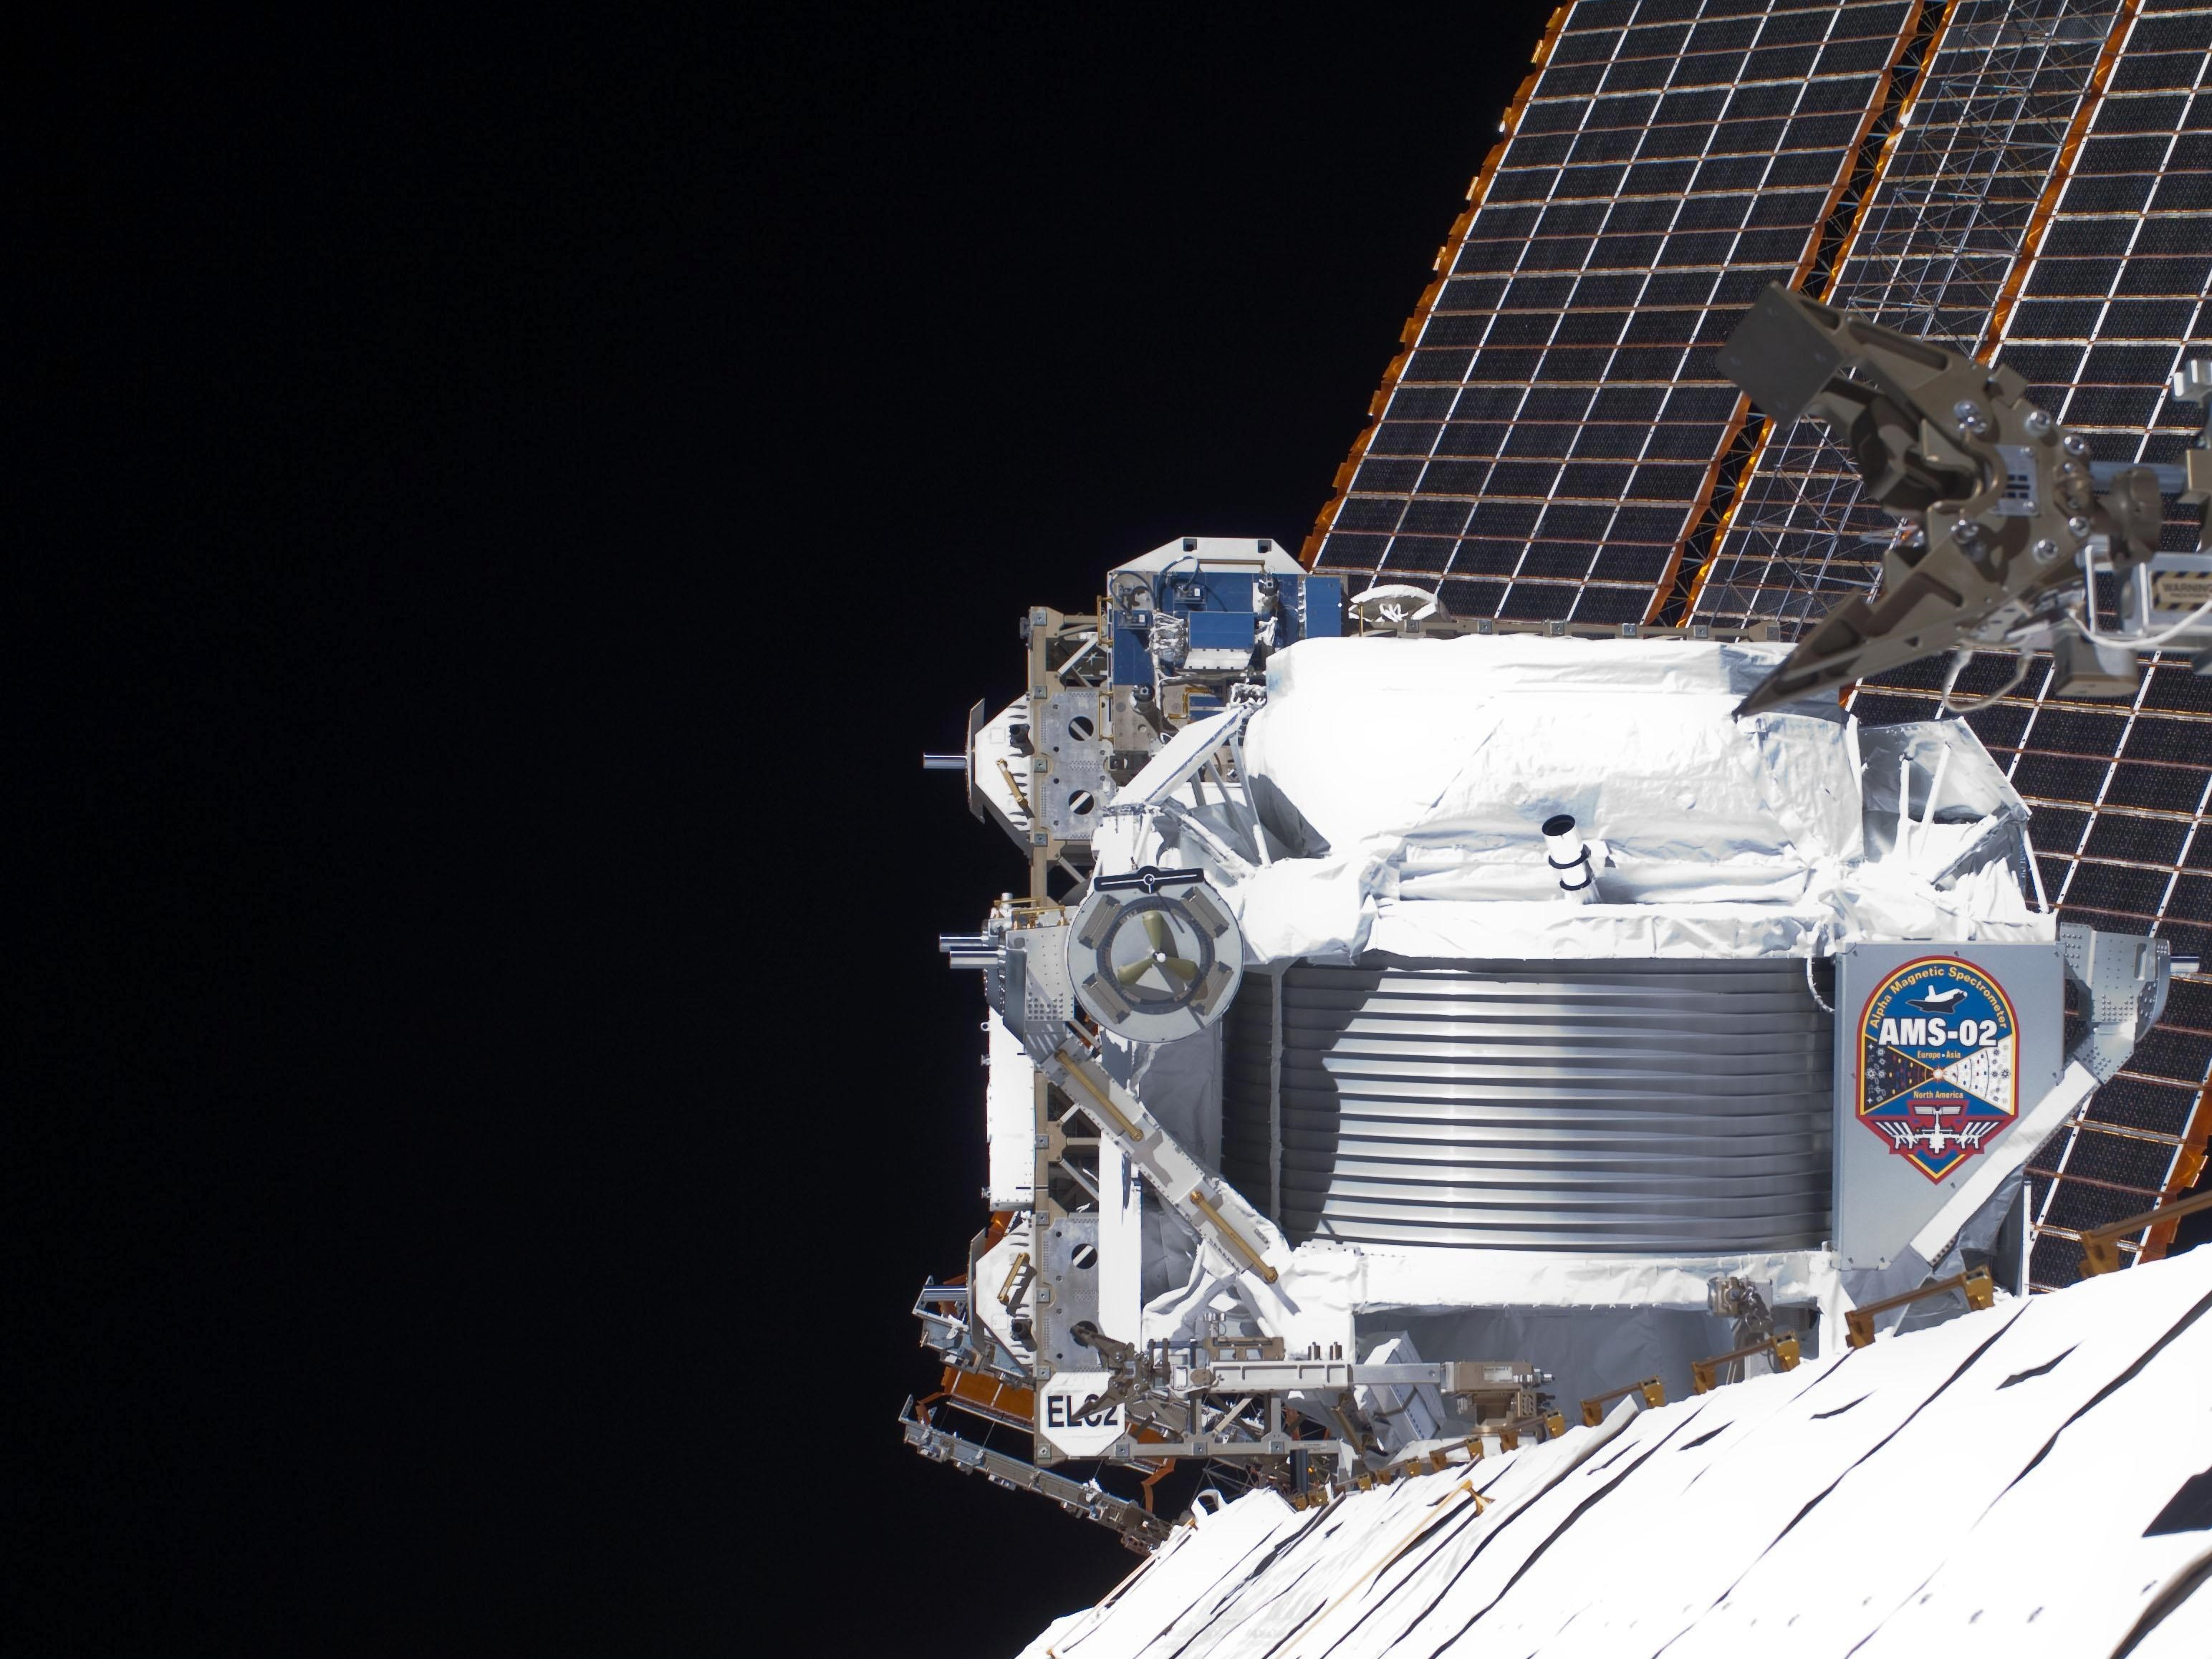
\includegraphics[height=\paperheight,keepaspectratio]{on_ISS-08_cutMIDDLEUP-3088.jpg}}	
	% 	possibili impostazioni per l'img: width=\paperwidth  --  height=\paperheight  --  keepaspectratio

\begin{frame}
	\titlepage
\end{frame}

\note{ 
\footnotesize{
The absorption thickness of the Earth's atmosphere, corresponding to an average of 25 radiation lengths (X0), screens the ground from primary CRs, which interact before reaching the detector. 

Direct detection of electromagnetically interacting CRs is therefore carried in space. In order to identify the nature of the detected particles, space borne instruments exploit typical high energy physics detection techniques, like um precision tracking using silicon detector technology or calorimetric energy measurements. 

Despite the detection concept is very similar to the modern accelerator experiments, the technological realization differs significantly. The requirements of a space borne experiment are in fact very challenging. Weight, dimension and power consumption constraints limit the size of the detector (thus their acceptance) to the $\sim$ 10 m$^3$ range. The limited bandwidth for the data transfer (to ground), the extreme thermal environment and the transport from ground to space also shape critically the detector concept.

In a typical direct CR detection experiment, particles traversing the instrument are fully characterized via the simultaneous measurement of the energy E, mass M, charge Z and charge sign. In a minimalistic experiment, a calorimeter is used to measure the energy E, dE=dX detectors are used to measure Z and a time of flight system is used to trigger the data acquisition and to measure the velocity and hence the mass M. A magnet can be used to detect the particle trajectory and infer the charge sign.

Some experiments are also equipped with additional detectors dedicated to the identification of CR rare species, like transition radiation detectors or neutron detectors that improve the identification of $e^{\pm}$. The measurement of CRs in space began in the 1970s with the measurement of nuclear isotopes in the energy range $\leqslant$ 1 GeV with the IMP satellites. The field flourished in 2000s, when the FERMI-LAT satellite observatory provided for the first time high precision rays direct measurements and the PAMELA satellite mission (see Figure 1.8) provided the direct measurement of charged CRs up to the 100 GeV range. The state-of-the-art space born experiment is the AMS-02 detector. AMS is the first particle detector located on the International Space Station (ISS) where it has been collecting high precision data up to the TeV range since 2011. The AMS detector will be exhaustively described in Chapter 2.

AMS successfully confirmed the possibility of operating a particle physics detector on the ISS, hence stimulating the development of the next (and ``next-to-next'') generation experiments to be operated on space stations, like the JEM-EUSO observatory or the DAMPE/HERD instrument.
}
}

\usebackgroundtemplate{}

\begin{frame}
\frametitle{Table of Contents}
\tableofcontents
\end{frame}

\begin{frame}
	\frametitle{Technical Question about the Detector}
	AMS is a particle physics experiment in space, so it focuses on the detection of particles, but:
	\begin{itemize}
	\item	Which kind of particle do we have to detect?
	\item	What is the required dimension of the detector?
	\item	Which ``property'' of the particle do we have to know?
	\begin{itemize}
		\item[$\circ$]	Position - Trajectory
		\item[$\circ$]	Time
		\item[$\circ$]	Number
		\item[$\circ$]	Energy
		\item[$\circ$]	Momentum
	\end{itemize}
	\item	What is the required resolution?
	\item	What is the maximum count rate?
	\item	What is the time distribution of the events?
	\item	And last, but not least, how much does it cost? 
	\end{itemize}
\end{frame}

\section{Introduction}
\begin{frame}
	\setbeamertemplate{background}{white}
	\frametitle{Introduction}
	\framesubtitle{The Alpha Magnetic Spectrometer}
	AMS-02 is a general purpose \textbf{high energy particle detector}  designed to operate as an external module on the International Space Station.
	
	\vspace{0.25cm}
	\begin{block}{Purpose of the AMS experiment}
		\justifying
		To perform accurate, high statistics, long duration measurements of the spectra of energetic primary charged 
		cosmic rays (CRs) in space. 
	\end{block}
		
	\vspace{0.25cm}
	Some of the \textbf{physics goals} are:
	\begin{enumerate}
		\item \bluetextbf{Dark Matter}
		\item \bluetextbf{Matter/Antimatter Asymmetry}
		\item \bluetextbf{Cosmic Ray Physics}
	\end{enumerate}
\end{frame}
\note{
	AMS-02 (Alpha Magnetic Spectrometer ) is a general purpose high energy particle detector which was successfully deployed on 
	the International Space Station (ISS) on May 19, 2011 to conduct a unique long duration mission of fundamental physics 
	research in space. Among the physics objectives of AMS are the searches for an understanding of Dark Matter, Anti-matter, the 
	origin of cosmic rays and the exploration of new physics phenomena not possible to study with ground based experiments
	Lo scopo dell'esperimento è quello di effettuare, per un periodo di lunga durata così da ottenere un'elevata statistica, delle 
	misure molto accurate dello spettro di energia (per energie fino all'ordine dei TeV) dei raggi cosmici carichi primari direttamente 
	nello spazio.
}

\section{Technical Requirements}
\subsection{from Physics Goals}
\begin{frame}
    \frametitle{Technical Requirements}
    \framesubtitle{from Physics Goals}
    
	Physical goals involve \textbf{technical requirements for the AMS detector}:
	
	\begin{itemize}
		\item	\bluetextbf{Dark Matter $\Rightarrow$}
					to get $e^+/p$ rejection of $\sim10^{-6}$ for the measurement of the positron fraction.
		\item	\bluetextbf{Matter/Antimatter Asymmetry $\Rightarrow$}
					to reach a sensitivity in the search for anti-matter nuclei of $10^{-10}$ (ratio of anti-helium nuclei to helium nuclei).
		\item	\bluetextbf{Cosmic Ray Physics $\Rightarrow$}
					to measure the composition and spectra of charged particles with an accuracy of 1\%.
	\end{itemize}
	
	Moreover, \bluetextbf{for each of these ones}, it is very important to extend, as far as possible, the energy range of the 
	measurements.
	
	For AMS, the required energy range is from 0.5 to $\sim$ 2000 $GeV$.

	%\footnotesize{\underline{\textbf{Note}} These requirements represent a considerable sensitivity improvement compared to the previous space-borne experiments.}

\end{frame}

\note{
	Esiste un forte interesse nell'effettuare delle misure di precisione della frazione di positroni dei raggi cosmici nella regione 
	energetica da 10 a 1000 GeV, in quanto le misurazioni di $e^+ / (e^+ + e^-)$, da AMS-01, HEAT, PAMELA e FERMI indicano 
	una grande deviazione di questo rapporto dalla produzione di e+ e e- previsto da un modello che comprende solo collisioni ordinarie del raggio cosmico.
   	 
   	These available measurements are both at too low an energy and of too limited statistics to shed the light on the origin of this 
   	significant excess.
   	 
	AMS-02 is expected to provide definitive answers concerning the nature of this deviation.
}

\begin{frame}
	\frametitle{Technical Requirements}
    \framesubtitle{from Physics Goals}	
    
    \begin{block}{The technical challenge of AMS-02}
		\justifying
		The illustrated requirements represent a considerable sensitivity improvement compared to the previous space-borne 
		experiments.
	\end{block}
   	
   	\vspace{0.25cm}
	\small{\bluetextbf{NOTE}}
	\vspace{-0.2cm}
    \begin{itemize}
    	\item[\footnotesize{$\blacktriangleright$}] 
    		\footnotesize{There is a strong demand for precision measurements of cosmic rays in the energy region from 10 to 1000 
    		$GeV$ as the measurements of positron fraction, i.e.  $e^+ / (e^+ + e^-)$, by AMS-01, HEAT, PAMELA and FERMI 
    		indicate a large deviation of this ratio from the production of $e^+$ and $e^-$ predicted by a model that includes only 
    		ordinary CR collisions.
    		
    		These available measurements are both at too low an energy and of too limited statistics to shed the light on the origin of 
    		this significant excess.
    		
    		AMS-02 is expected to provide definitive answers concerning the nature of this deviation.}
   	\end{itemize}  
   	 
%
%%	\vspace{0.25cm}
%	There is a strong demand for precision measurements of cosmic rays in the energy region from 10 to 1000 GeV as the 
%	measurements of e+/(e+ + e-) by AMS-01, HEAT, PAMELA and FERMI indicate a large deviation of this ratio from the 
%	production of e+ and e- predicted by a model that includes only ordinary cosmic ray collisions. 
%	
%	These available measurements are both at too low an energy and of too limited statistics to shed the light on the origin of this 
%	significant excess. 
%	
%	AMS-02 is	expected to provide definitive answers concerning the nature of this deviation.
\end{frame}

%\begin{frame}
%	\frametitle{Technical Requirements}
%    \framesubtitle{From Physics Goals}
%	\begin{columns}
%		\begin{column}{0.5\textwidth}
%			\begin{center}
%				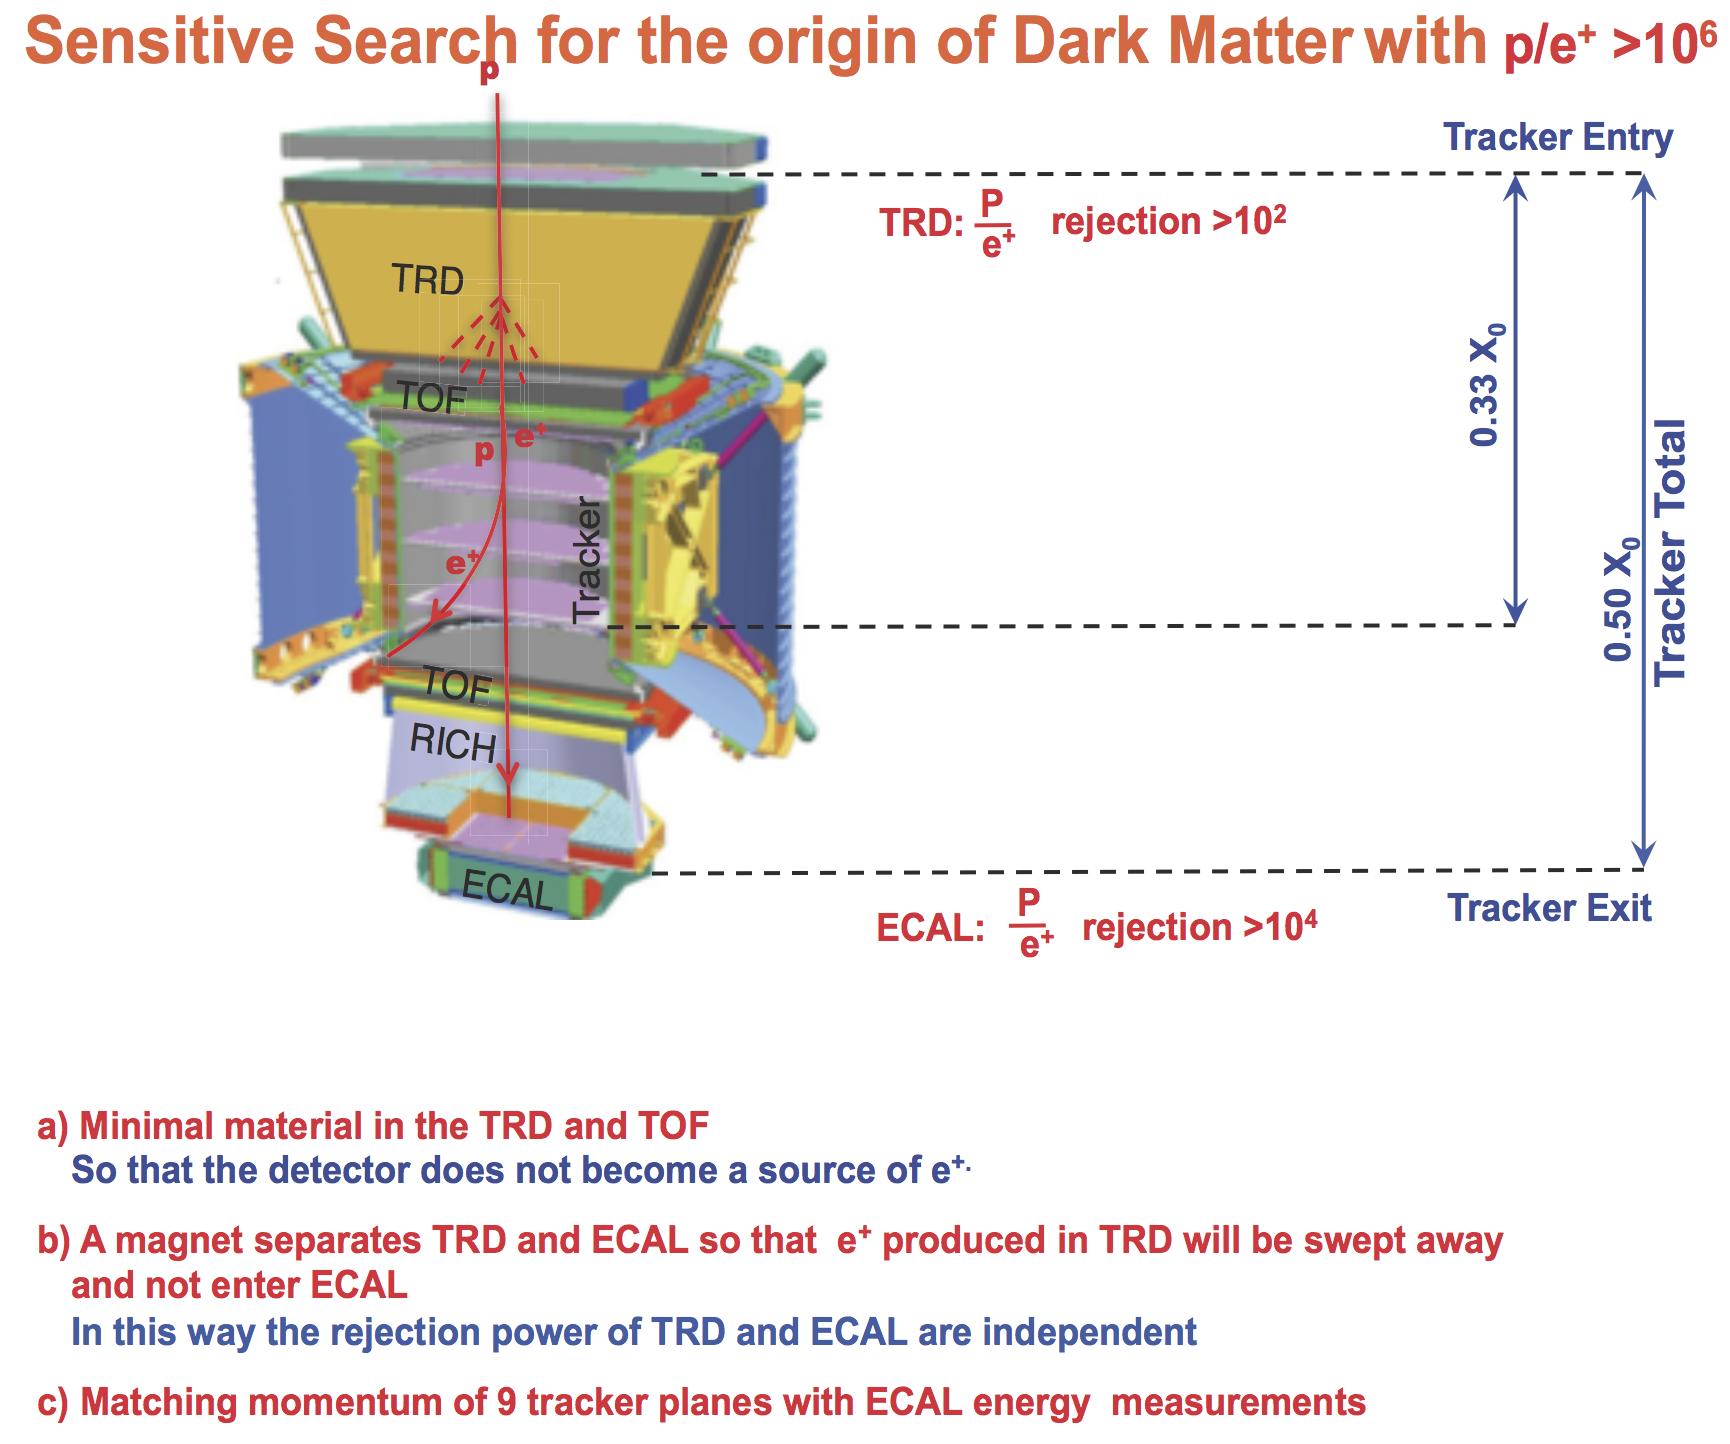
\includegraphics[width=0.95\columnwidth]{Schem_Requirements-DM.png}
%			\end{center}
%		\end{column}
%
%		\begin{column}{0.5\textwidth}
%			\begin{center}
%				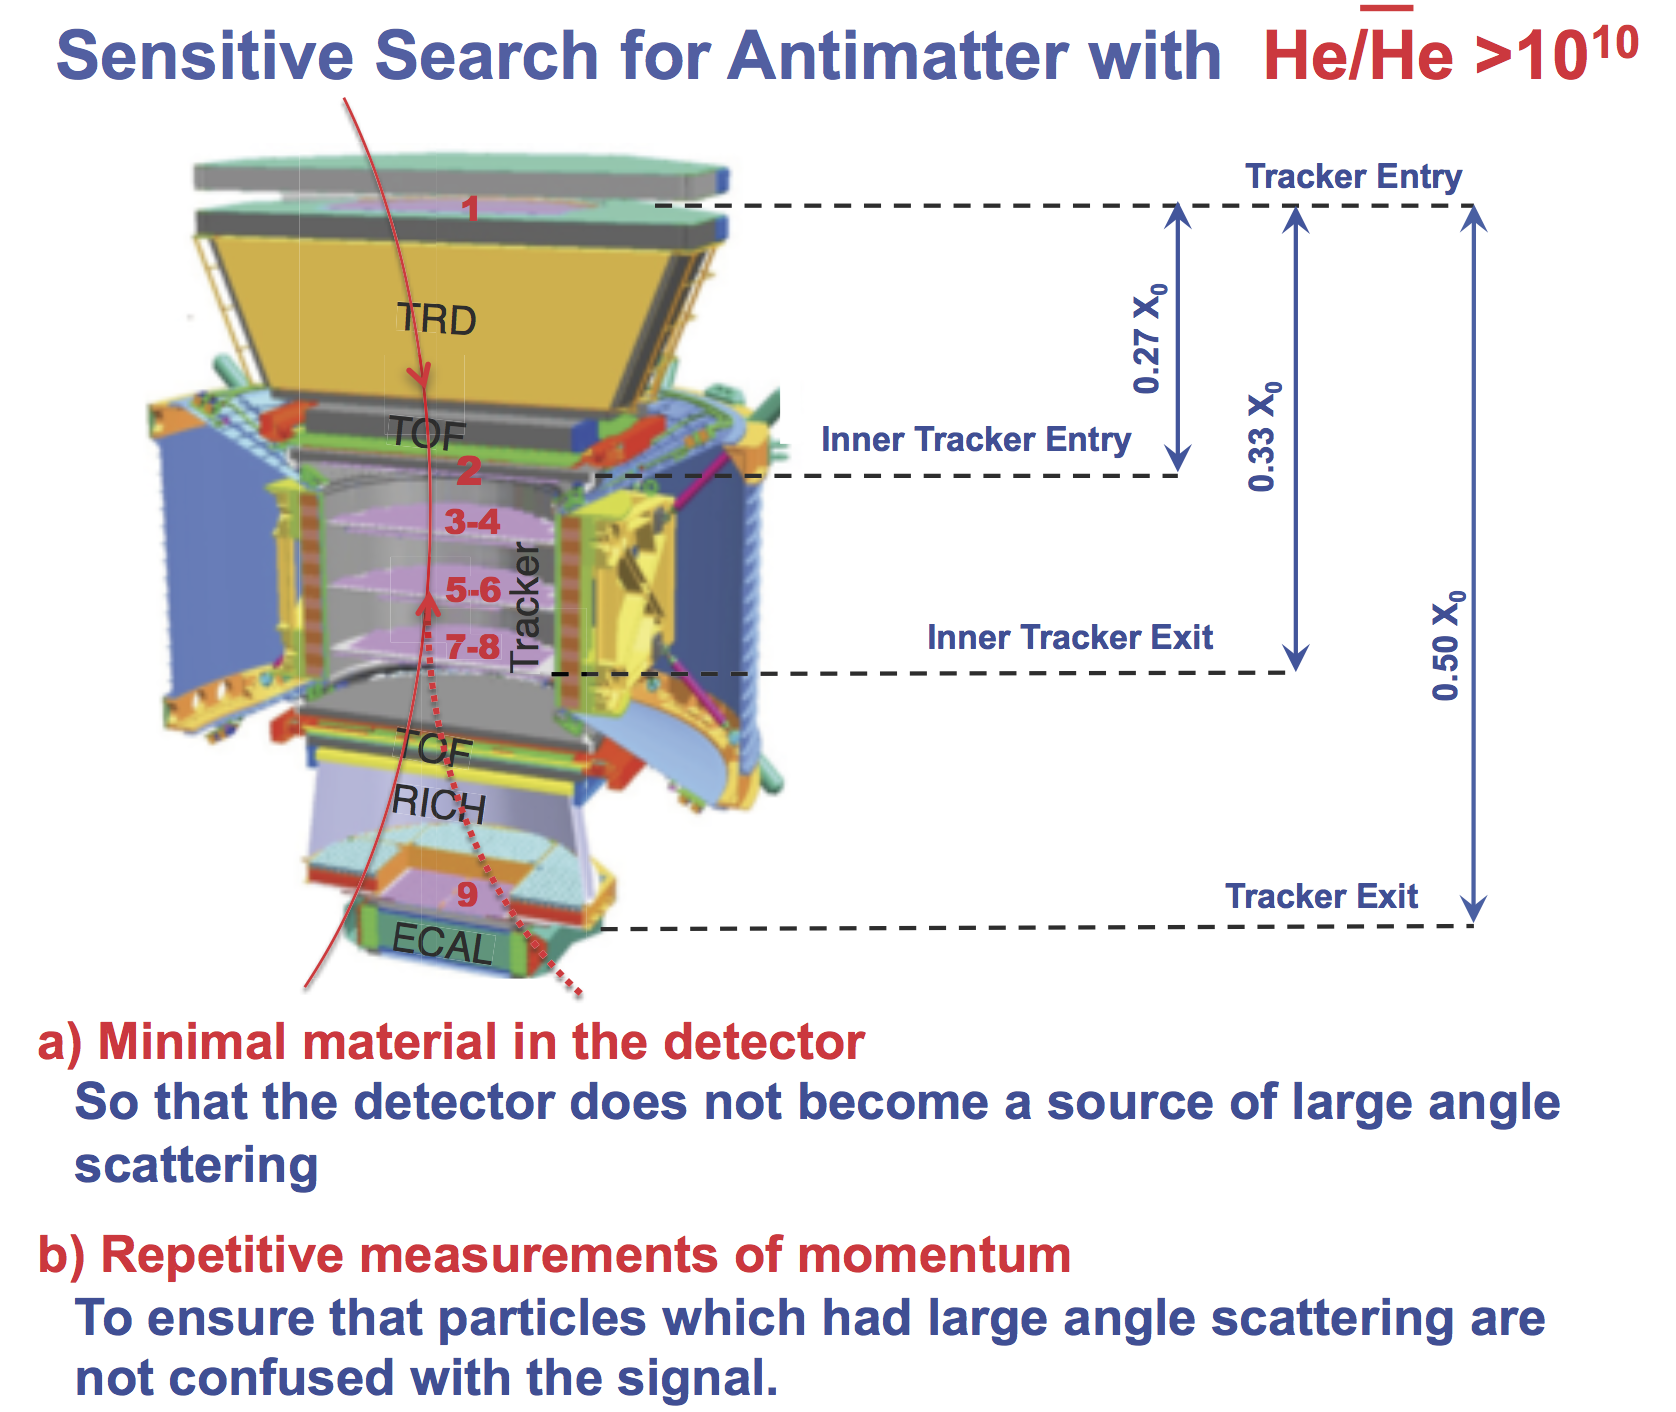
\includegraphics[width=0.95\columnwidth]{Schem_Requirements-Antimatter.png}
%			\end{center}
%		\end{column}
%	\end{columns}
%\end{frame}

\begin{frame}
	\frametitle{Technical Requirement}
	\framesubtitle{general structure of the AMS apparatus}
	\begin{center}
		\vspace{-0.45cm}
		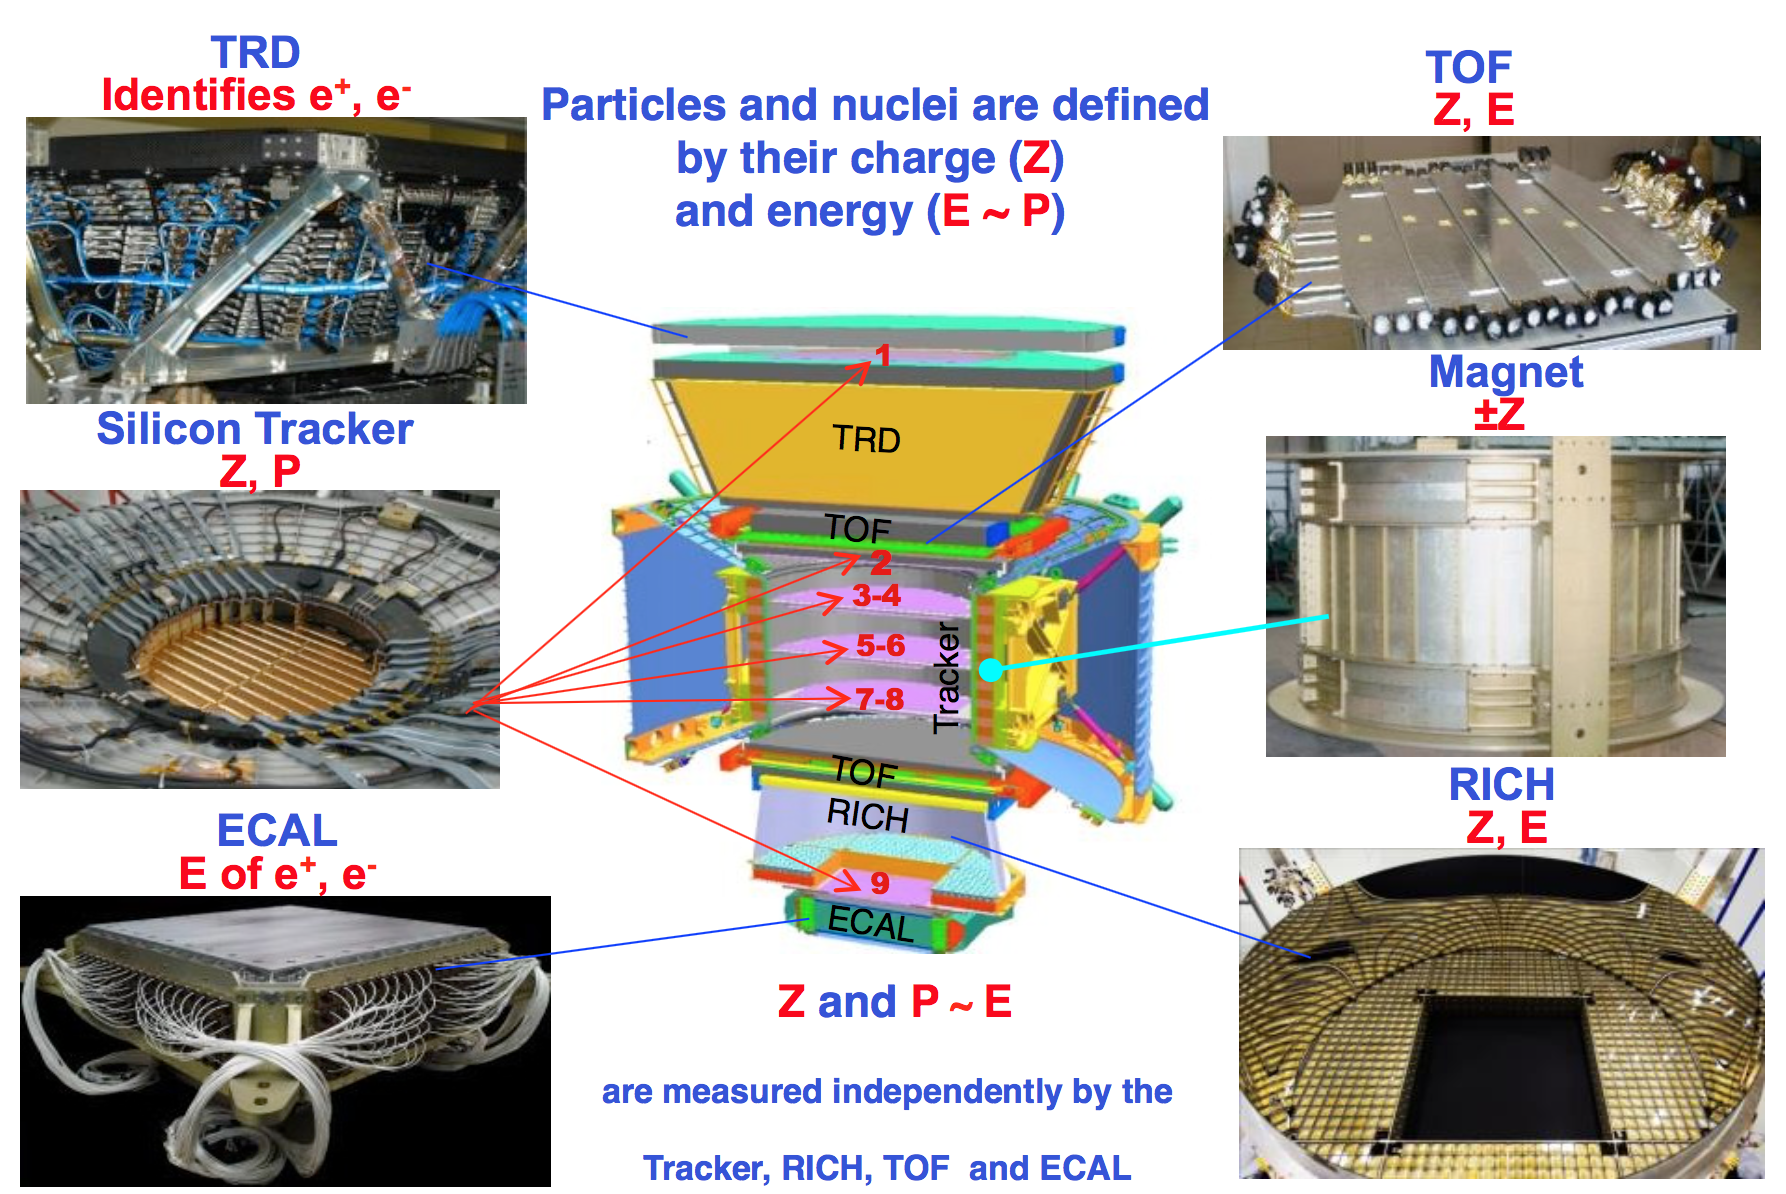
\includegraphics[height=0.7\paperheight]{Schem_structure_of_AMS-02.png}
	\end{center}
\end{frame}

\begin{frame}
	\frametitle{Technical Requirement}
	\framesubtitle{from the research on the Dark Matter}
	\begin{center}
		\vspace{-0.1cm}
		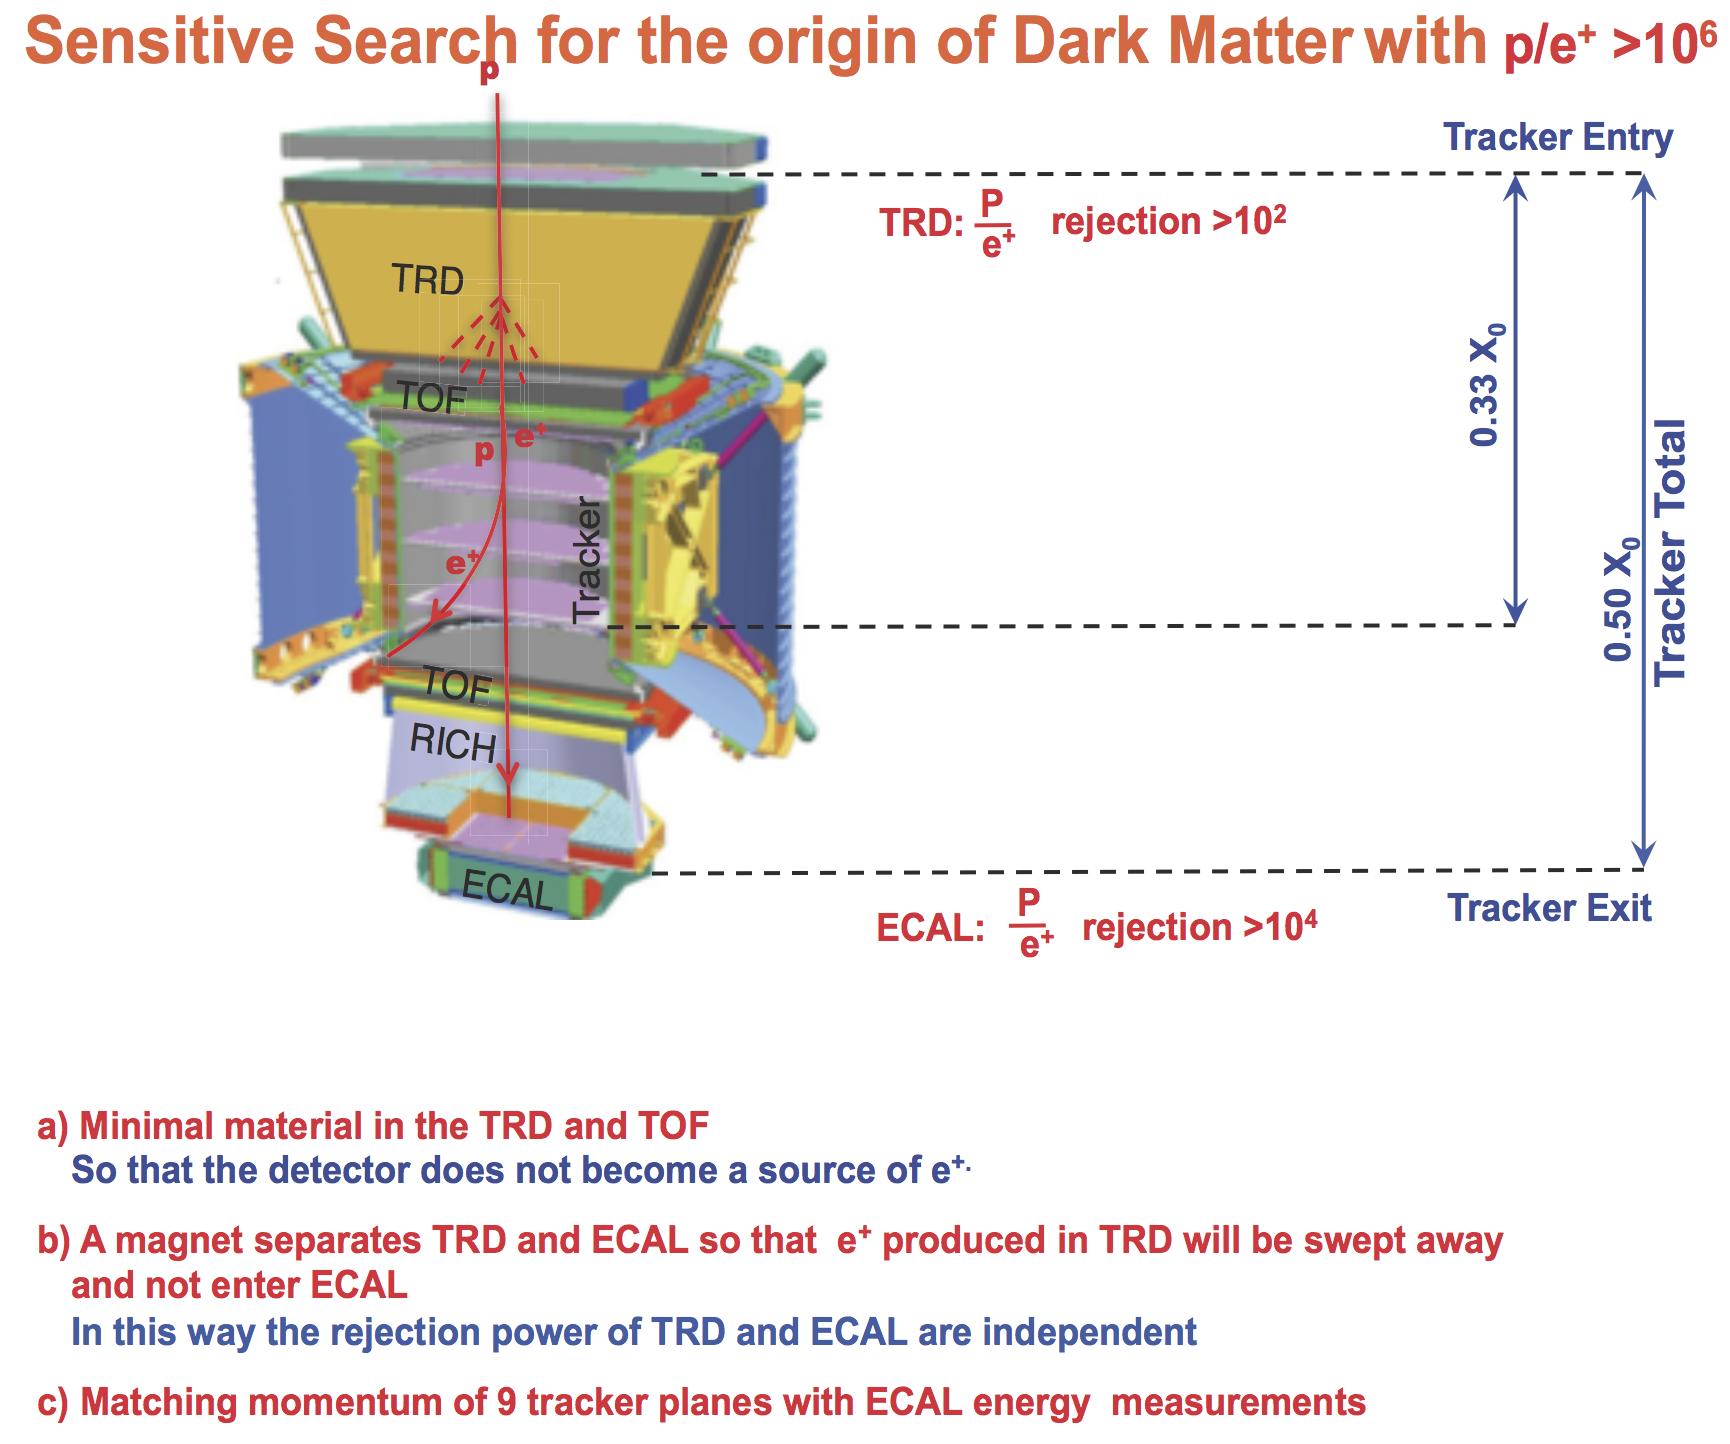
\includegraphics[height=0.72\paperheight]{Schem_Requirements-DM.png}
	\end{center}
\end{frame}

\begin{frame}
	\frametitle{Technical Requirement}
	\framesubtitle{from the research on the Matter/Antimatter Asymmetry}
	\begin{center}
		\vspace{-0.1cm}
		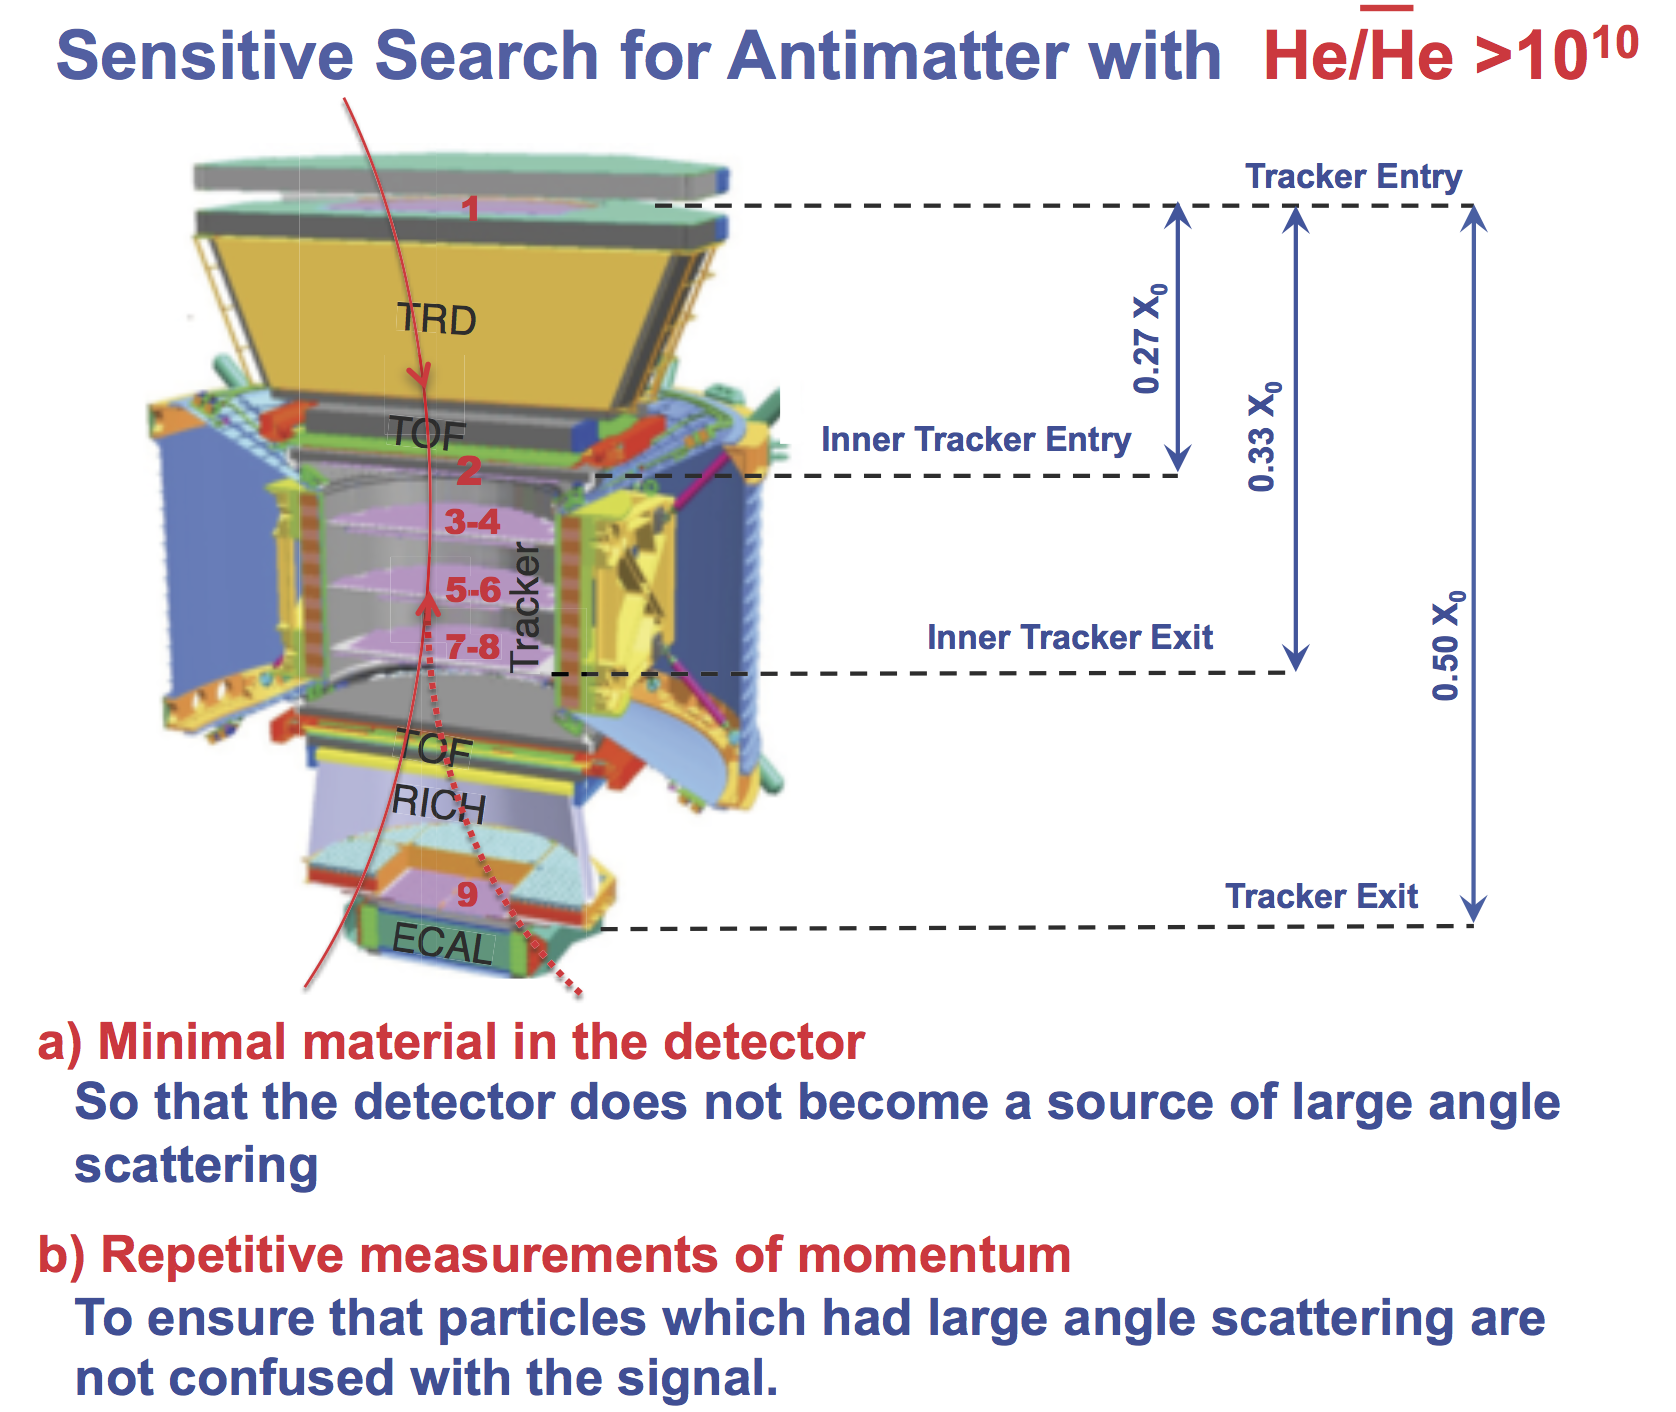
\includegraphics[height=0.65\paperheight]{Schem_Requirements-Antimatter.png}
	\end{center}
\end{frame}

\begin{frame}
	\frametitle{Technical Requirement}
	\framesubtitle{from the research on the Cosmic Ray}
	\begin{center}
		\vspace{-0.5cm}
		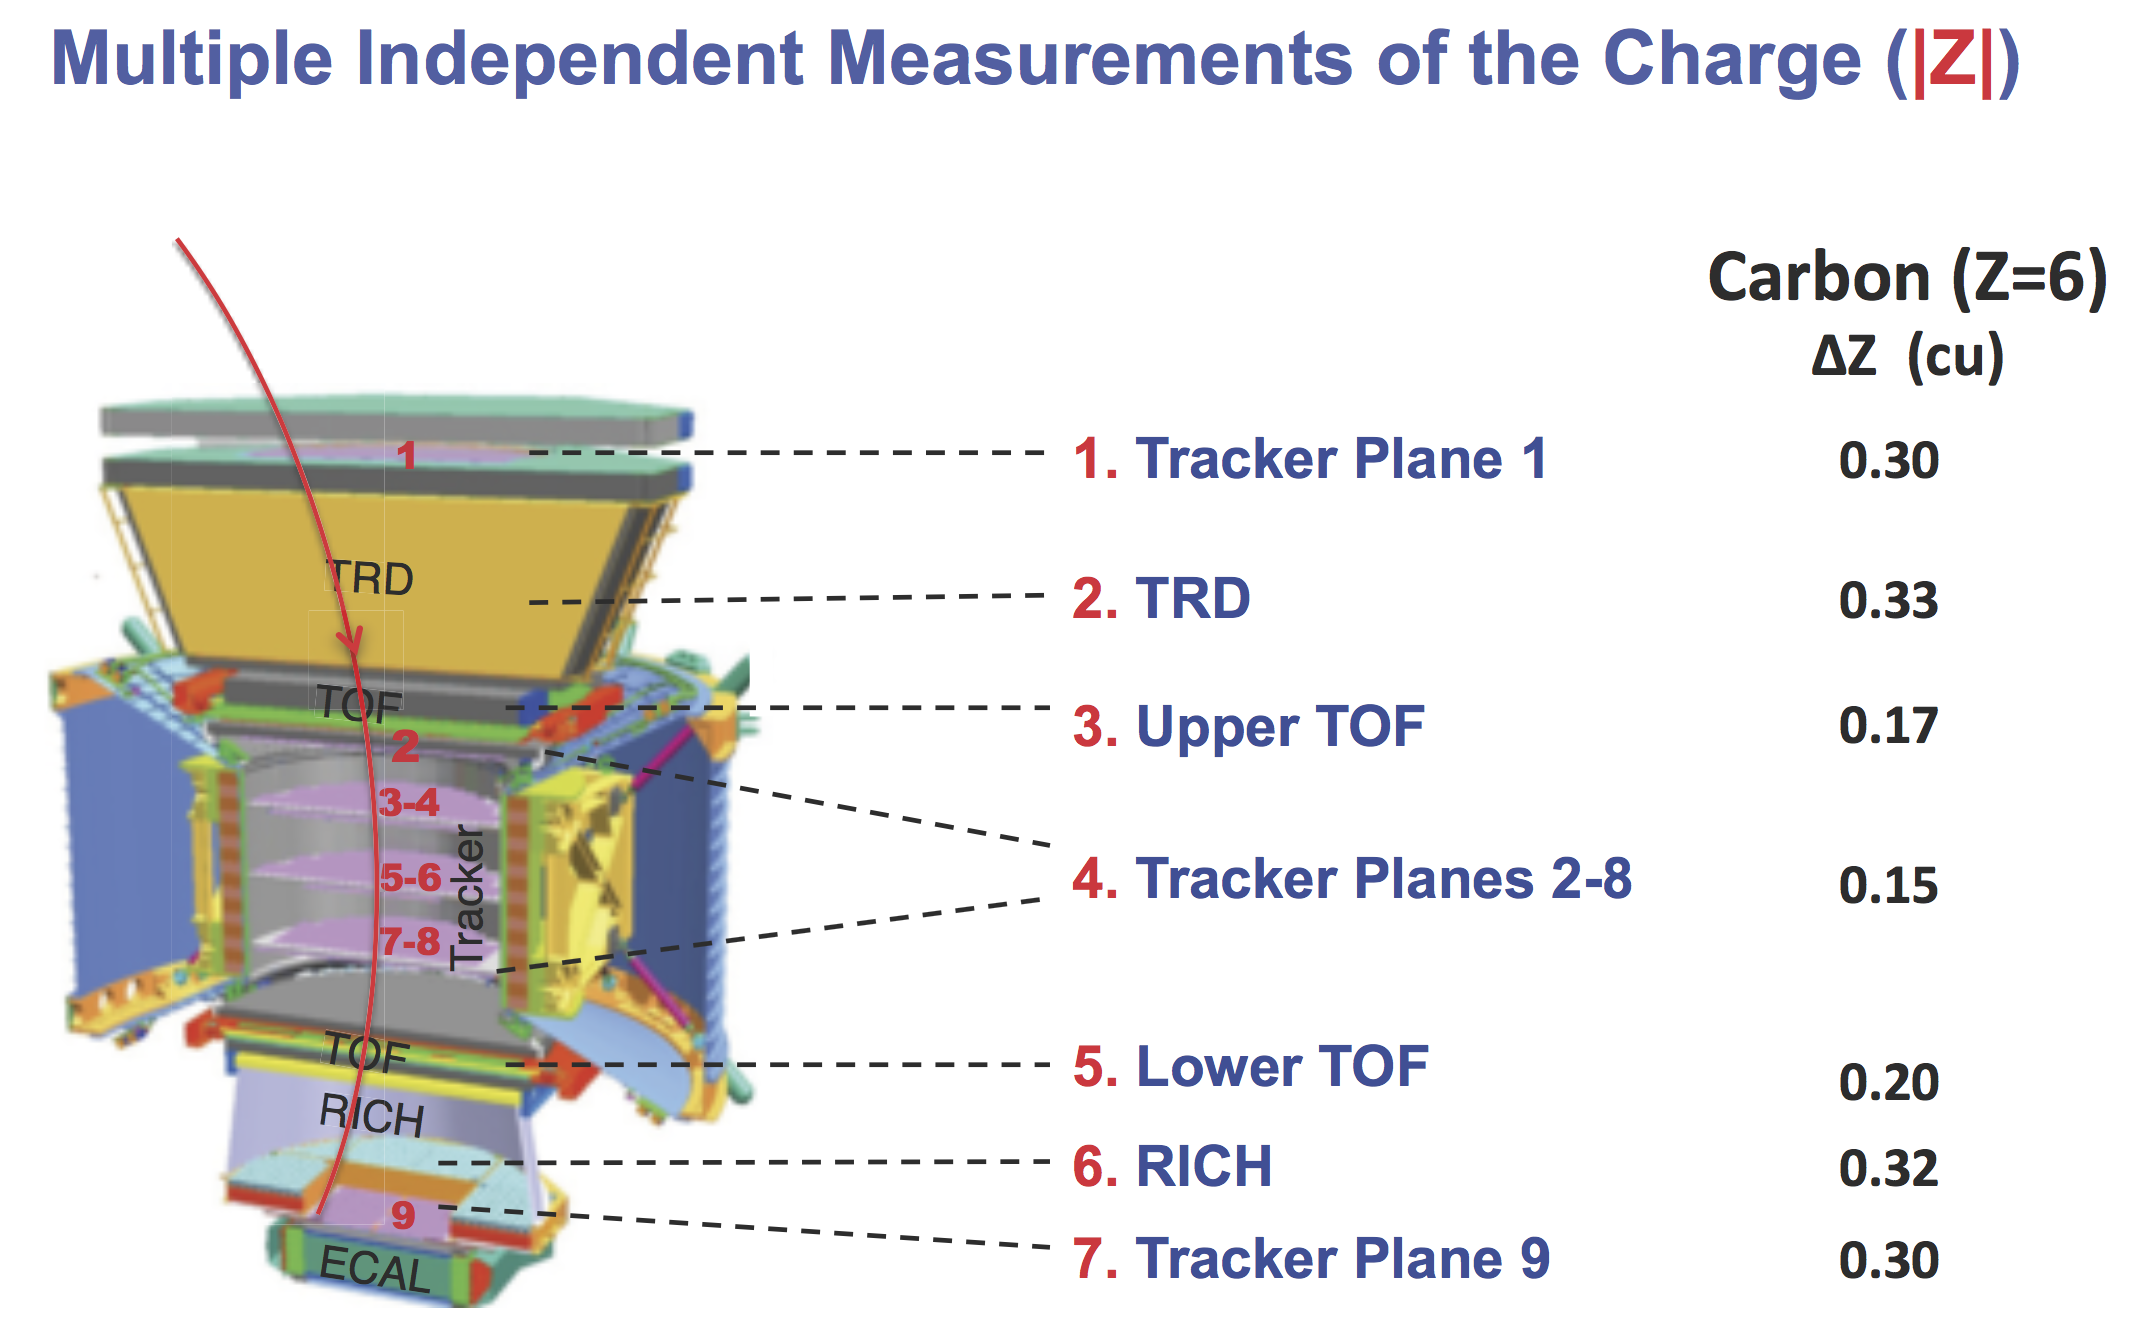
\includegraphics[height=0.55\paperheight]{Schem_Requirements-Charge02.png}
	\end{center}
\end{frame}

%\begin{frame}
%	\frametitle{Technical Requirement}
%	\framesubtitle{From the research on the Cosmic Ray}
%	\begin{center}
%		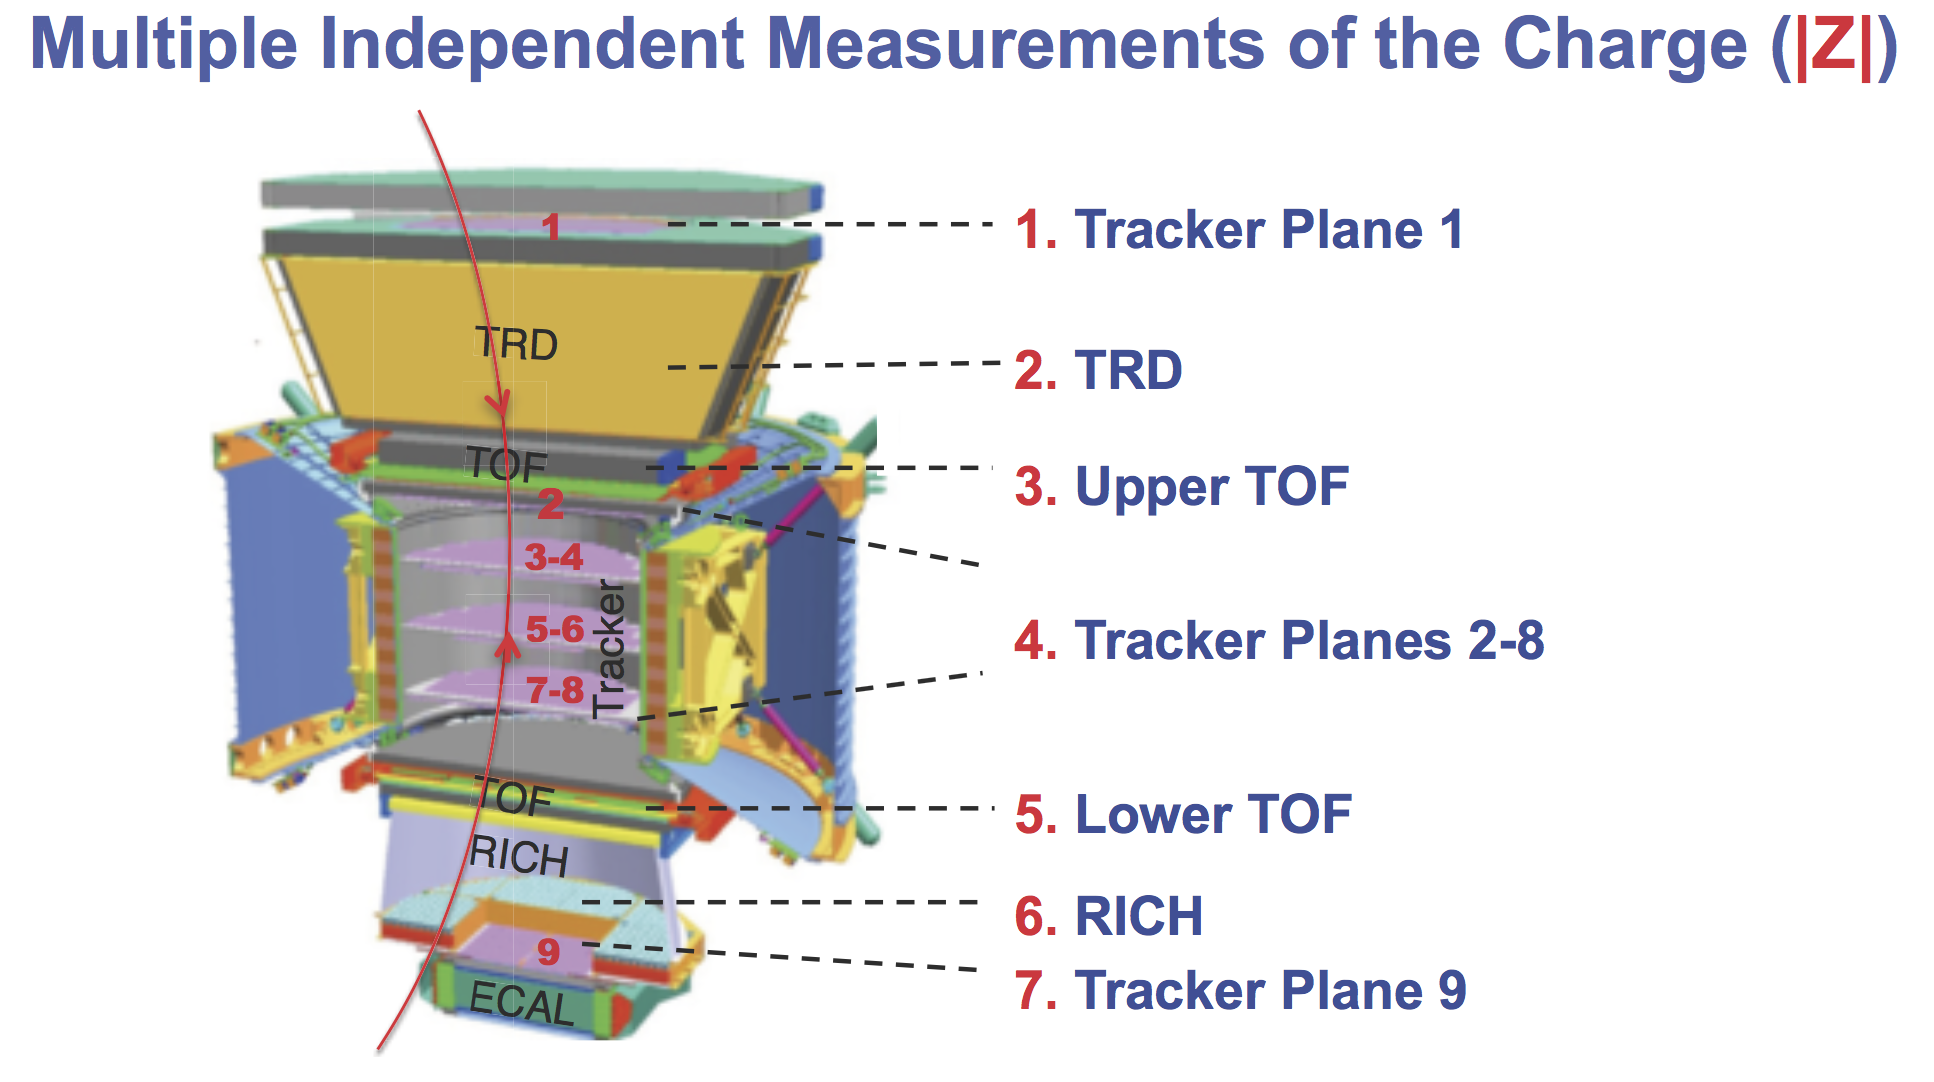
\includegraphics[height=0.5\paperheight]{Schem_Requirements-Charge.png}
%	\end{center}
%\end{frame}

\subsection{space-borne experiment}
\begin{frame}
	\frametitle{Particle Detector in Space} 
	\framesubtitle{The challenge of a space-borne experiment}
	
The absorption thickness of the Earth's atmosphere, corresponding to an average of 25 radiation lengths (X0), screens the ground from primary CRs, which interact before reaching the detector. 

Direct detection of electromagnetically interacting CRs is therefore carried in space. In order to identify the nature of the detected particles, space borne instruments exploit typical high energy physics detection techniques, like um precision tracking using silicon detector technology or calorimetric energy measurements. 

\end{frame}

\begin{frame}
	\frametitle{Technical Requirement} 
	\framesubtitle{of a space-borne experiment}

Despite the detection concept is very similar to the modern accelerator experiments, the technological realization differs significantly. The requirements of a space borne experiment are in fact very challenging. Weight, dimension and power consumption constraints limit the size of the detector (thus their acceptance) to the $\sim$ 10 m$^3$ range. The limited bandwidth for the data transfer (to ground), the extreme thermal environment and the transport from ground to space also shape critically the detector concept.

\end{frame}

\begin{frame}
	\frametitle{Technical Requirement} 
	\framesubtitle{of a space-borne experiment}
	New environment for HEP experiments
	\begin{itemize}
		\item	Operation in vacuum
		\item	Acceleration during start and landing up to 9g
		\item 	Temperature variations from $-180^\circ C$ to $+50 ^\circ C$
		\item	Deposition limits on ISS $< 10^{-14} \frac{g}{s \cdot cm^2}$
		\item	Weight limited to 13500 lb
		\item	Datarate $1 Mbyte/s$ via 1 datalink
		\item	Power consumption limited to 2kW
		\item	Powersupply at 120 V via 1 powercable
		\item	Redundancy
	\end{itemize}
\end{frame}

\subsection{the protype (AMS-01)}
\begin{frame}
	\frametitle{AMS-01} 
	\framesubtitle{The protype of AMS-02}
	%In order to ensure that technologies used in the detector construction work reliably in space, a scaled down detector 
	(AMS-01) was built and flown in 1998 onboard the STS-91 mission for 10 days.
	Before installation on the Space Station, AMS performed an engineering flight on the Space Shuttle to ensure that:
	
	\begin{itemize}
		\item	The AMS experiment can function properly in space; in vacuum with orbital temperature changes from -65 to 40 
					$^{\circ}$C and in the intense radiation background (which contains heavy nuclei causing single event latch-up in 
					chips).
		\item	The detector can withstand the tremendous vibrations (150 dB) and acceleration (3 g) at launch and the 
					deacceleration (6.5 g) at landing;
	\end{itemize}

	This mission was subsequently referred to as AMS-01.
\end{frame}

\begin{frame}{The Numbers of AMS-02}
	\begin{itemize}
	\small{
	\item[$\circ$]	\textbf{Weight}: 8500 kg
	\item[$\circ$]	\textbf{Volume}: 64 cubic meters
	\item[$\circ$]	\textbf{Power}: 2500 watts
	\item[$\circ$]	\textbf{Data downlink}:  9 Mbps (average)
	\item[$\circ$]	\textbf{Magnetic field intensity}: 0.15 Tesla (4.000 times stronger than the Earth magnetic field)
	\item[$\circ$]	\textbf{Magnetic material}: 1200 kg of Neodymium alloy (Nd$_2$Fe$_{14}$B)
	\item[$\circ$]	\textbf{Subsystems}: 15 among particle detectors and supporting subsystems
	\item[$\circ$]	\textbf{Launch}: 16th May 2011, 08:56 am EDT
	\item[$\circ$]	\textbf{Mission duration}: through the lifetime of the ISS, until 2024 or longer (it will not return back to Earth)
	\item[$\circ$]	\textbf{Construction}: 1999-2010
	\item[$\circ$]	\textbf{Cost}: \$ 1.5 billion (estimated)
	}
	\end{itemize}
\end{frame}

\section{The subdetectors of AMS-02}
\begin{frame}{The AMS-02's subdetectors}{from the top to the bottom}	
	\begin{itemize}
		\item	\textitem{TRD}{Trasition Radiation Detector}, identifies electrons and positrons among other CRs.
		\item	\textitem{ToF}{Time of Flight}, warns the sub-detectors of incoming CRs.
		\item	\bluetextbf{Magnetic Spectrometer}, detects the particle charge sign, separating matter from antimatter. Main 
					components:
								\begin{itemize}
									\item[$\circ$]	\textcolor{itemblue}{Magnet}, bends in opposite directions charged particles/
															antiparticles.
									\item[$\circ$]	\textcolor{itemblue}{Silicon Tracker}, direct measurement of the trajectory deflection.
								\end{itemize}
		\item	\textitem{RICH}{Ring-Imaging CHerenkov detector}, measures with high precision the velocity of CRs.
		\item	\textitem{ECAL}{Electromagnetic CALorimeter}, measures energy of incoming electrons, positrons and $\gamma$-rays.
	\end{itemize}
\end{frame}

\subsection{TRD}
\begin{frame}{TRD - Transition Radiation Detector}%{Particle ID \& 3D tracking}
	\vspace{-0.55cm}
	\begin{center}
	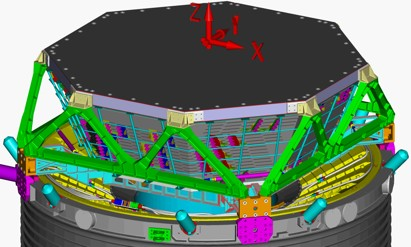
\includegraphics[height=0.35\paperheight]{TRD-Photo-05.jpeg}
	\end{center}
	\vspace{-0.45cm}
	\begin{block}{\small{The main features of TRD are:}}
		%\vspace{-0.25cm}
		\begin{itemize}\small{
			\item[$\circ$] to discriminate between  $e^+$ and $p$ whit a proton rejection of $10^{-2} \div 10^{-3}$ 
						in the energy range between $10$ and $300 GeV$.$^1$
						
			\item[$\circ$] to identify the nuclei by measurement of the charge $|Z|$.
		}\end{itemize}
%		\vspace{-0.55cm}
%		\begin{center}
%			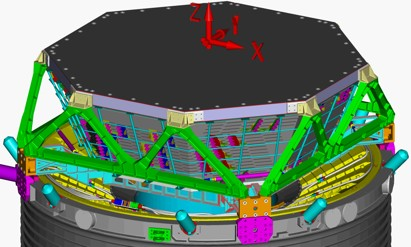
\includegraphics[height=0.35\paperheight]{TRD-Photo-05.jpeg}
%		\end{center}
	\end{block}
	\footnotetext[1]{This seems that, even if $e^+$ and $p$ 
						have the same charge, and so they are somewhat similar (i.e. in the other sub-detector, apart for the ECAL, 
						$e^+$ and $p$ with different energy give the same signals and therefore they may be confused), TRD may
						wrongly interpreter a $p$ as an $e^+$ only every $100 \div 1000$ real $p$ events.}
\end{frame}

\begin{frame}{TRD - Transition Radiation Detector}{the exploited physical process}
	\begin{columns}%[T]
	
		\begin{column}{0.5\textwidth}
			\justifying
			\small{The operating principle of TRD is mainly based on the known physical phenomenon, predicted by Ginzburg and 
			Frank in 1946 and observed, for the first time, by Goldsmith and Jelley in 1959, named:}
			
			\vspace{0.25cm}
			\begin{block}{Transition Radiation (TR)}
				\justifying
				TR is the electromagnetic radiation that is emitted whenever a charged particle transverse the interface 
				between two media with different refractive indexes.
			\end{block}
		\end{column}
		
		\begin{column}{0.5\textwidth}
			\begin{center}
%				\vspace{-0.75cm}				%		se l'allignamento delle colonne è impostato su [T]
				\vspace{-0.4cm} 				%		se l'allignamento delle colonne non è impostato su [T]
				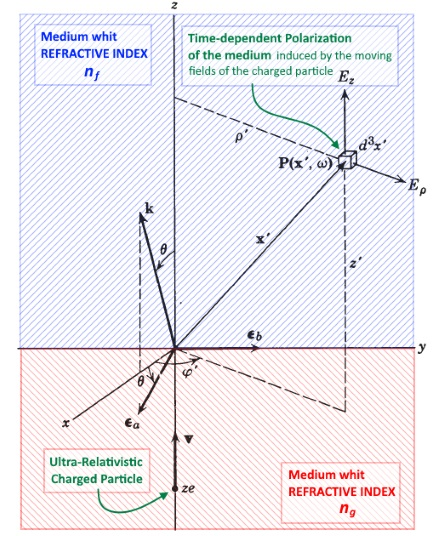
\includegraphics[width=0.9\columnwidth]{TransitionRadiation-ColorVers02mid.jpg}
			\end{center}
		\end{column}
		
	\end{columns}
\end{frame}

\begin{frame}[label=TRD-main]
	\frametitle{TRD - Transition Radiation Detector}
	\framesubtitle{the main features of transition radiation process}

	\begin{itemize}
		\small{
			\item \textbf{The emission spectrum of TR depends on the traversed material and on the particle's energy.} 
					 Typically, this emission phenomena is relevant for ultra-relativistic particle ($\gamma \geqslant 300$) 
					 and the emitted photon are soft X-rays (i.e. they have an energy of the order of a few $KeV$).
			\item \textbf{Total energy emitted per interface crossed is proportional to $\gamma$} and therefore 
					 to the $E/mc^2$ ratio.
			\item \textbf{Number of emitted TR photons per interface crossed is small}, 
					 e.g. for a unit charge $\sim (3 \cdot 137)^{-1}$
			\item Particle must traverse a minimum distance, the so-called 
					 \textbf{formation zone $D_f$}, in order to efficiently emit TR.
			\item Very small emission angle: $\theta \lesssim \gamma^{-1}$. \textbf{TR photons stay close to particle's track.}
		}
	\end{itemize}
%	\begin{columns}
%		\begin{column}{0.65\textwidth}\end{column}
%		\begin{column}{0.35\textwidth}
%			\hyperlink{TR-details}{\beamerbutton{click here for more details on TR}}
%		\end{column}
%	\end{columns}
	\hfill \hyperlink{TR-details}{\beamerbutton{click here for more details on TR}}
\end{frame}

\begin{frame}{TRD - Transition Radiation Detector}{based on a well-proven design }
Since the particle momentum is determined with the AMS-02 silicon tracker by measuring the trajectory inside the magnet, the detected transition radiation (TR) can be used to distinguish between particles of different masses, like positrons and protons.

	\begin{columns}
		\begin{column}{0.4\textwidth}
			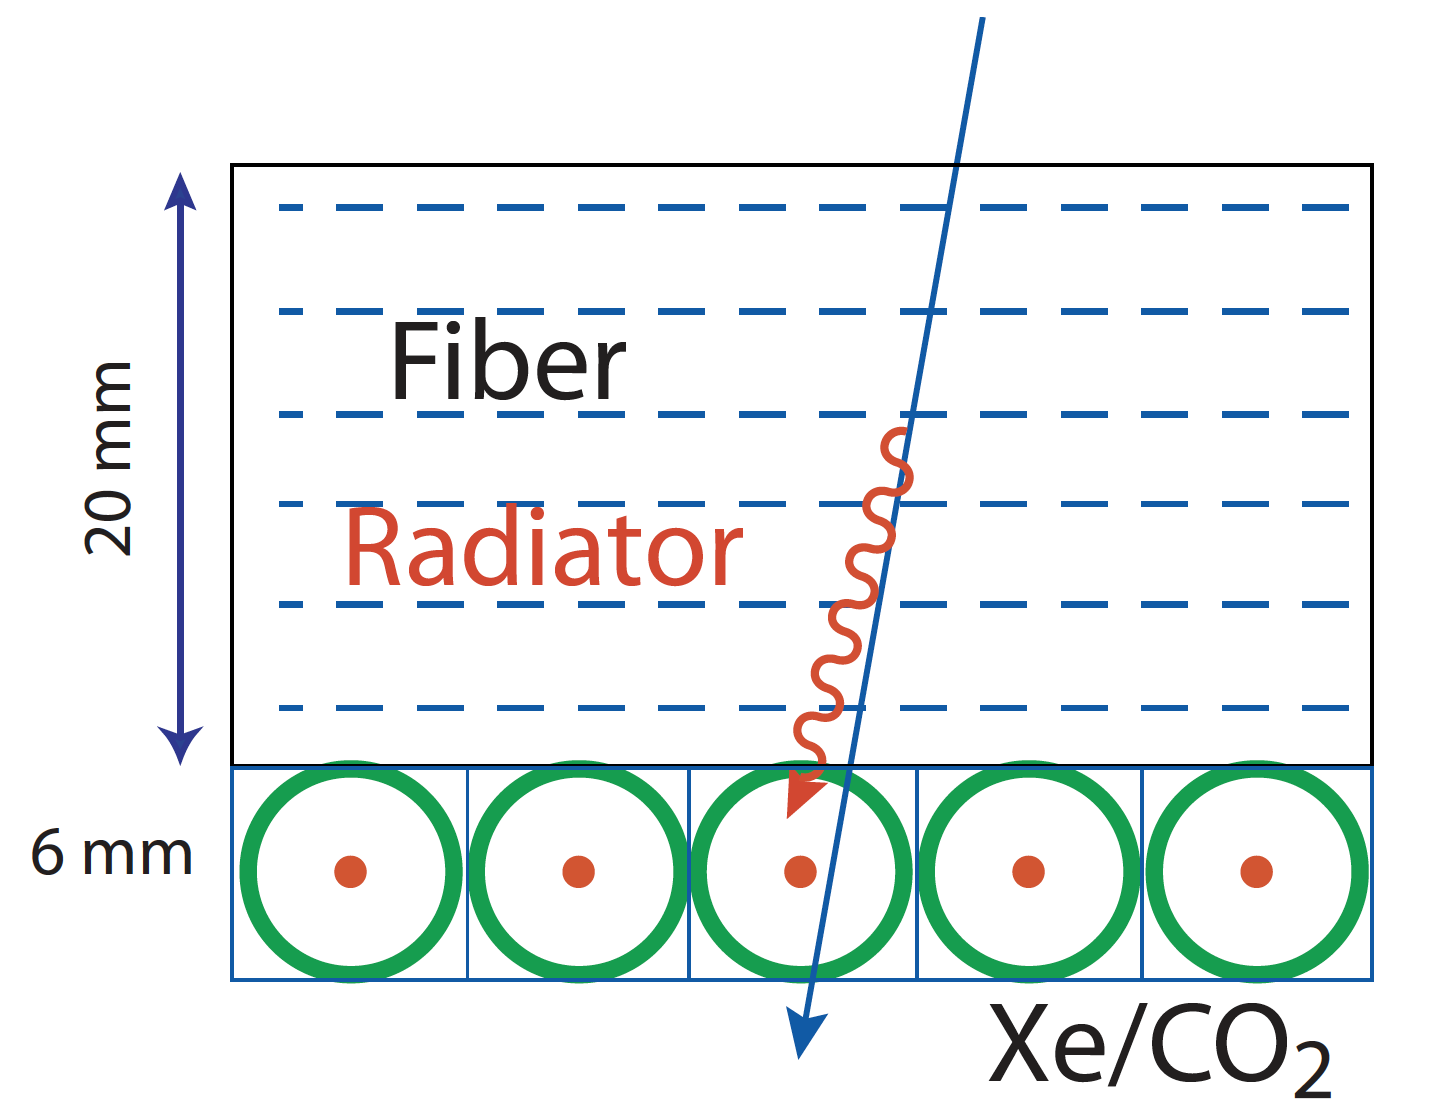
\includegraphics[width=0.9\columnwidth]{TRD-Stack.png}
		\end{column}
		\begin{column}{0.6\textwidth}
			The AMS-02 TRD is based on a well-proven design with multiple irregular boundary crossings in a 20-mm fleece radiator and straw tube proportional wire chambers filled with $\text{Xe} / \text{CO}_2$ gas to detect the TR-photons. The TRD consists of 20 layers of fleece and straw tube modules.
		\end{column}
	\end{columns}

\end{frame}

\begin{frame}
The challenge is to build such a detector in a space-qualified way with strict limits on outgassing, gas tightness, weight and power consumption whilst assuring safety and gas gain homogeneity in a harsh environment during payload lift and in orbit without the possibility of further access to the experiment. This involves detailed finite-element calculations as well as subcomponent vibration and thermo-vacuum-cycle tests. The optimized AMS-02 TRD design with 2m diameter and with 5248 straw tubes weighs less than 500 kg.
\end{frame}

\begin{frame}{Others sub-system of the AMS-02 experimet}{}
	\begin{itemize}
		\item	\textitem{ACC}{Anti-Coincidence Counter}, rejects CRs traversing the magnet walls.
		\item	\textitem{TAS}{Tracker Alignment System}, checks the Tracker alignment stability.
		\item	\bluetextbf{Star Tracker and GPS}, defines the position and orientation of the AMS-02 experiment.
		\item	\bluetextbf{Electronics}, transform the signals detected by the various particle detectors into digital information to be analysed by computers.
	\end{itemize}
\end{frame}


\begin{frame}[label=TR-details]
	\frametitle{TRD}
	\framesubtitle{Transition Radiation Detector}
	\hyperlink{TRD-main}{\beamerbutton{back to TRD}}
	\footnotesize{
	\begin{equation*} 
		\frac{dW}{d\omega} = \frac{Z^2 \alpha}{\pi} \left[ \frac{\epsilon_f^2 + \epsilon_g^2 + 2 \gamma^{-2}}{\xi_f^2-\xi_g^2}	\ln \left( \frac{\gamma^{-2} + \epsilon_f^2}{\gamma^{-2} + \epsilon_g^2} \right) - 2 \right]
	\end{equation*}
	
	\begin{equation*}
		\frac{dW}{d\omega} \simeq \frac{Z^2 e^2}{6 \pi c} \left( \frac{\omega_c}{\omega} \right)^4
	\end{equation*}
	
	\begin{equation*}
	\frac{dW}{d\omega} \simeq \frac{2 Z^2 e^2}{\pi c} \ln \left( \frac{\omega_c}{\omega} \right)
	\end{equation*}
	
	\begin{equation*}
	\frac{dW}{d\omega} \simeq \frac{2 Z^2 e^2}{\pi c} \left[ \ln \left( \frac{\omega_c}{\omega} \right) - 1 \right]
	\end{equation*}
	
	\begin{equation*}
		W_{TR} \simeq Z^2 \cdot \frac{\hbar \omega_p}{3\cdot 137} \cdot \gamma \propto Z^2 \cdot \frac{E}{m c^2}
	\end{equation*}
	\begin{equation*}
		\theta_{TR} \lesssim \gamma^{-1}
	\end{equation*}
	\begin{equation*}
		D_{f} \simeq \frac{2 c}{\omega \left( \gamma^{-2} + \theta_{TR}^2 + \xi^2 \right)}
	\end{equation*}
	}
\end{frame}

\end{document}
